\chapter{Studi Literatur}

Bab ini akan berisi pembahasan dari studi literatur yang akan berkaitan dengan permasalahan yang dibahas di Tugas Akhir ini.
Hasil studi literatur akan menjadi dasar dalam pengerjaan Tugas Akhir ini baik untuk menganalisis masalah dan juga untuk merancang solusi.

\section{Distributed Tracing}

\subsection{\textit{Overview} Distributed Tracing}
Dengan meningkatnya penggunaan Microservice, cara untuk melakukan \textit{profiling}, \textit{debugging}, dan \textit{monitoring} aplikasi menjadi berbeda dengan cara yang dilakukan pada aplikasi yang berbentuk Monolith.
Salah satu cara untuk melakukan profiling pada aplikasi berbasis Microservice adalah dengan Distributed Tracing.
Distributed Tracing, disebut juga dengan Distributed Request Tracing, adalah sebuah tipe logging terkorelasi yang dapat memberikan pengguna mendapatkan visibilitas pada operasi dari perangkat lunak terdistribusi untuk kasus seperti debugging di environment \textit{production}, dan analisis penggalian akar masalah pada kegagalan atau insiden lainnya \citep{parker2020distributed}.
Dengan adanya kakas Distributed Tracing, pengguna dapat mendapatkan insight mengenai operasi yang terjadi di aplikasi terdistribusi secara kolektif dengan cara melakukan pelacakan pada \textit{request} yang dibuat oleh suatu \textit{service}.

Kita bisa sebut setiap pekerjaan yang dilakukan oleh sebuah \textit{service} dalam suatu waktu sebagai \textit{span}.
Setiap \textit{span} bisa diisi dengan \textit{metadata}, seringkali disebut sebagai \textit{attributes} atau \textit{tags}, dan \textit{events}, seringkali disebut sebagai \textit{logs}.
Setiap pemanggilan Remote Procedure Call (RPC) atau Application Programming Interface (API) antara \textit{service} akan merepresentasikan hubungan dari \textit{request} yang terjadi diantara \textit{service} tersebut.
Hubungan tersebut disebarkan diantara \textit{service} sebagai \textit{trace context}, yaitu data yang secara unik mendefinisikan \textit{span} yang dibuat oleh setiap \textit{service}.
Setiap \textit{span} yang dibuat oleh setiap \textit{service} tersebut diteruskan kepada proses eksternal yang dapat dikumpulkan atau diagregasi sebagai sebuah \textit{trace}.
\textit{Trace} tersebut dapat dianalisis lebih lanjut dan disimpan untuk mendapatkan \textit{insight} mengenai \textit{service}.
Berikut adalah ilustrasi sederhana mengenai \textit{trace}:
\begin{figure}[htb]
      \centering
      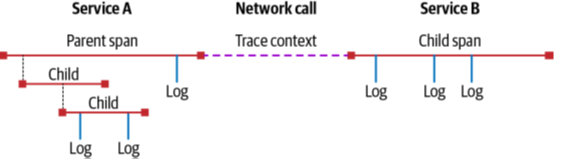
\includegraphics[width=0.6\textwidth]{resources/ch2/tracing-illus.png}
      \caption{Ilustrasi Tracing}
      \label{TracingIlllustration}
\end{figure}

Adapun komponen-komponen yang membangun sistem Distributed Tracing adalah sebagai berikut \citep{parker2020distributed}:
\begin{enumerate}
      \item Instrumentasi \\
            Distributed Tracing membutuhkan data \textit{trace} agar dapat bekerja.
            Data \textit{trace} dihasilkan dengan cara menginstrumentasikan proses-proses \textit{service} atau mentrasformasikan data telemetri yang sudah ada ke data \textit{trace}.
      \item \textit{Deployment} \\
            Setelah data \textit{trace} dihasilkan, kita perlu mengirimkan data tersebut ke suatu tempat.
            Melakukan \textit{deployment} pada sistem \textit{tracing} membutuhkan pemahaman dimana perangkat lunak kita dijalankan di \textit{server} dan bagaimana perangkat tersebut dijalankan.
            Agar dapat memaksimalkan kemampuan dari \textit{tracing} juga meminimalkan \textit{overhead} yang terjadi pada aplikasi, kita perlu memahami teknik yang cocok untuk melakukan deployment pada sistem Distributed Tracing yang akan kita gunakan.
      \item Penyampaian \textit{Value} \\
            Saat \textit{service} kita telah dapat menghasilkan data \textit{trace} dan kita telah memiliki infrastruktur yang diperlukan untuk mengolah data \textit{trace} tersebut, kita akan memerlukan kakas yang tepat untuk menggabungkan \textit{trace} dari berbagai \textit{service} dengan metadata lain seperti \textit{metrics} dan \textit{logs} untuk dapat menghasilkan \textit{value} yang berguna bagi proses \textit{debugging}, \textit{profiling}, dan \textit{monitoring} perangkat lunak terdistribusi.
\end{enumerate}

\subsection{Instrumentasi Distributed Tracing}

\subsection{\textit{Deployment} Distributed Tracing}

\subsection{Penyampaian \textit{Value} Distributed Tracing}

\subsection{Pelacakan \textit{request causality}}

\section{Protokol Komunikasi Micro\textit{service}}
Pada subbab ini akan dijelaskan beberapa protokol komunikasi yang bisa digunakan dalam arsitektur Microsevice.
\subsection{REST API}
Representational State Transfer (REST) merupakan sebuah gaya arsitektur yang dibuat untuk mendesain sistem yang berjalan di World Wide Web.
REST pertama kali diperkenalkan oleh Roy Thomas Fielding dalam disertasinya pada tahun 2005 yang berjudul \textit{Architectural Styles and the Design of Network-based Software Architectures}.
Dalam mendesain arsitektur, REST mendefinisikan beberapa aturan yaitu skalabilitas antara komponen yang berinteraksi, antar muka yang seragam, \textit{deployment} yang independen bagi komponen, dan pembuatan arsitektur berlapis yang dapat memfasilitasi komponen untuk melakukan \textit{caching} agar dapat mengurangi \textit{latency}, memperkuat \textit{security}, dan mengenkapsulasi sistem \textit{legacy} \citep{rest}.

\subsection{GraphQL}
\subsection{gRPC}
Berikut adalah contoh Kode gRPC:
\lstinputlisting[captionpos=b, caption={Contoh File Proto}]{codes/ch2/hello.proto}

\subsection{WebSocket}


\section{Kubernetes}


\section{Penelitian Terkait}